The data that is received from the sensors generates a continuous data stream for every sensor. A good feature representation of the data is required so that the LDA model can be applied. The feature representation that is described in this chapter is used as the artificial words for the LDA model that is described in chapter \ref{chapter:topic_models} about the Topic model.
First the data is divided into five fields and all the sensors in one field are grouped together. In this way the data is reduced to five dimensions. 
The continuous data stream cannot be used as input for the LDA model. Like it is done in the work of Farrahi \cite{farrahi2008daily} the data of one day is divided into time-slices of length $l$. If for example the length of the time-slices is $l=30$ min., the number of time-slices on one day is $n=48$. For a chosen number of the time-slices $n$ the length of time-slices for one day can then be calculated with $l=1440/n$ in minutes. In the experiments (chapter \ref{chapter:experiments}) the number of time-slices is varied to see the effect on the topic model.
A day starts and ends at 3 a.m. in the morning. In this way the chance to cut between activities is reduced. It still can occur that a person goes to bed late or that he needs to visit the toilet. For now this fact is left out in the part of modeling.\\

For every time-slice the number of sensor activations of one field are counted. In one time-slice for each sensor field the number of times is counted that the signal changes from zero to one. The duration of an active signal, thus for how long a sensor field has the value one, is not taken into account. This is done because for example a door that accidentally is left open would otherwise generate a high value although this value is not very informative and would though disturb the data. Then the observations contains a high value but does not contain a lot of information about the behavior.
Every sensor field then builds a dimension of the observations $o_n$. In figure \ref{fig:FeatEx} an example on how the data is translated into a vector representation is given for one time-slice.

\begin{figure}[h]
\centering
\begin{minipage}{0.55\linewidth}
\centering
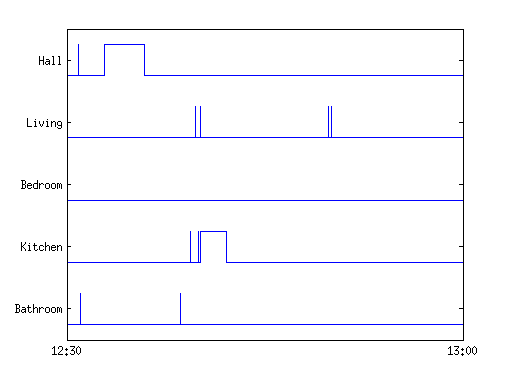
\includegraphics[width=\textwidth]{Pictures/FeatExample.png}
\label{fig:FeatEx}
\end{minipage}
\begin{minipage}{0.35\linewidth}
\centering
\begin{equation*}
o_n = 
 \begin{bmatrix} 
 o_{Hall}\\
 o_{Living}\\
 o_{Bedroom}\\
 o_{Kitchen}\\
 o_{Bathroom}\\
 o_{time}
 \end{bmatrix}
 =
  \begin{bmatrix} 
 2\\
 4\\
 0\\
 3\\
 2\\
 t
 \end{bmatrix}
\end{equation*}
\end{minipage}
\caption{Vector representation of the data. The data of the sensors is shown in the left image. It is translated in the vector shown on the right-hand side.}
\end{figure}

The last dimension of the observation $o_n$ represents the time value of the given time-slice. There are two different ways how the time dimension is added to the observations. The fine-grain representation adds the number of the time-slice in which an observations is captured, at the end of the observation vector. In the coarse-grain representation, which is also used in the work Farrahi \cite{} and Castanedo \cite{}, the 24 hours of a day are divided into the five time intervals $\{ 3am - 8am, 8am - 1pm, 1pm - 18pm, 18pm - 23pm, 23pm - 3am  \}$. So the observation of figure \ref{fig:FeatEx} will become $o_n=\{2,4,0,3,2,2\}$ in the coarse-grain representation. The observation falls into the second time interval. In the fine-grain representation the observation will be $o_n=\{2,4,0,3,2,20\}$ if the total number of time-slices on a day is $n=48$.\\




If the number of time-slices is set to $n=48$ the maximal value that is observed in one field is 28. This is an extreme value and occurs not that often in the data. If the maximum value for each field is set to 15 and the time is coarse grain, there are approximately 4 million ($10^5*5$) possible observations that can be made. As a comparison: In the work of Farrahi \cite{} only 512 ($4^3*8$) different observations are possible and 2856 days of data for 68 people is available.\\
In table \ref{tab:features} an overview is given how many unique words are actual observed for the different houses and how many words are totally observed ($48*\text{\# of days}$). One can see that the number of unique observations scales with the number of days available for each house. This shows that there are a lot of unseen observations in the data.\\


\begin{table}
 \centering
 \begin{tabular}{l c c c c c}
  HouseNr & 1 & 2 & 3 & 4 & 5\\
  \hline
  \# of days & 142 & 98 & 89 & 63 & 73 \\
  words & 6816 & 4704 & 4272 & 3024 & 3504 \\
  unique words & 2147 & 1644 & 1764 & 1068 & 1087\\
 \end{tabular}
 \caption{}
 \label{tab:features}
\end{table}


The given feature representation, with the two variation of the time dimensions, fine grain and coarse grain, are used in the following chapters. There are much more possibilities to describe the feature. An overview of different possibilities is given in the Future work (chapter \ref{chapter:future_work}).

%Every field of the observation has a different distribution on how often an activity of the 
%In figure ... an overview of the distribution of the values of the five fields is shown. For house number one the observation 
% EVENTUEL nog histograms of one house toevoegen